\chapter{Evaluation}

Im diesem letzten Teil der Arbeit sollen die beiden Implementierungen der Algorithmen evaluiert und miteinander verglichen werden.
Für die Evaluation sollen die Algorithmen das CEP-System Heron über das implementierte Framework kontrollieren, während ein möglichst realitätsnaher Strom von Tupeln vom System abgearbeitet werden muss.

Das folgende Kapitel gliedert sich in mehrere Teilbereiche.
Zuerst müssen Daten erhoben werden, die während der Evaluation vom System verarbeitet werden müssen.
Hierzu wurden Tweets von der Twitter-Streaming API ausgelesen und gesichert.
Diese reflektieren realitätsnahe Schwankungen des Arbeitsaufwandes.
Anschließend wird der Systemaufbau für die Evaluation durchgeführt.
Außerdem wird kurz die Wahl von Heron als System für die Evaluation und dessen spezielle Eigenschaften erläutert.
Für die Evaluation ist zudem eine Topologie notwendig.
Diese definiert wie die im ersten Schritt erhobenen Daten während der Evaluation verarbeitet werden.
Dazu wurde speziell für die Evaluation eine neue Topologie entwickelt, die Tweets einliest und anschließend analysiert.
Im darauf folgenden Teil werden die in den vorherigen Kapiteln beschriebenen Parameter der Algorithmen für die Evaluation definiert und deren Wahl begründet.
Anschließend wird noch ein kurzer Überblick über den Ablauf der Evaluation gegeben.

Zum Ende des Kapitels wird die Evaluation der Algorithmen mit den erhaltenen Messwerten  durchgeführt.
Das Ziel ist dabei, dass die Algorithmen auf Basis der Parallelisierungsgrade, der Tupel-Latenz und der Fehlerrate von Tupeln miteinander verglichen werden.
So kann der Schluss gezogen werden, welcher Algorithmus die Topologie während der Analyse der vorliegenden Daten besser gesteuert hat.


\section{Testdaten}
Um einen realitätsnahen Datenstrom erzeugen zu können, wurden während dem August 2018 Tweets von der Twitter-Streaming API abgerufen und gespeichert.
Neben kostenpflichtigen Schnittstellen bietet die API kostenlos einen kontinuierlichen Datenstrom von zufällig gewählten Tweets.
Die gewählten Tweets sind dabei für jeden Konsumenten, der sich für den Datenstrom registriert hat, identisch \cite{noauthor_get_nodate}.
Der Datenstrom liefert ca. 1\% der gesamten anfallenden Twitter-Daten in Realzeit \cite{noauthor_how_2017}.
Dies sind neben neuen Statusupdates (Tweets) auch Löschanfragen zu bestehenden Tweets.
Aus Gründen der besseren Lesbarkeit werden im Folgenden beide Arten der Statusänderung als Tupel bezeichnet.
Für die Evaluation werden die gesammelten Tupel der Woche vom 7. - 13. August 2018 verwendet.

In dieser Zeit wurden 32.416.487 Tupel erfasst die ca. 160 GB Textdaten entsprechen.
Die Abbildung 9.1 zeigt die Verteilung der Anzahl erfasster Tupel pro Stunde im Verlauf der Woche.
Beginn der Aufzeichnung ist Dienstag, 07.08.2018 00:00 UTC.


\begin{figure}
 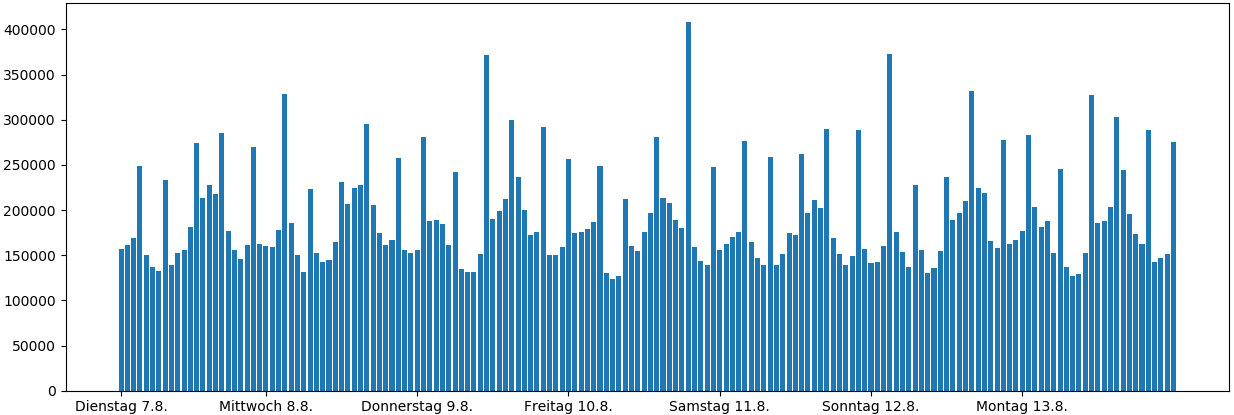
\includegraphics[scale=0.45]{Twitter-Daten.png}
 \caption{Anzahl Tupel pro Stunde.}
\end{figure}

\section{Systemaufbau}
Die Evaluation wurde auf dem internen OpenStack-Cluster des Instituts für Verteile und Parallele Systeme der Universität Stuttgart durchgeführt.
Für die Evaluation wurde ein Cluster aus vier virtuellen Maschinen aufgebaut.
Die Maschinen werden mit dem Betriebssystem Ubuntu 14.04 betrieben.
Drei der virtuellen Maschinen sind je mit 24 CPU-Kernen, 32 GB Arbeitsspeicher und 50 GB persistentem Speicher ausgestattet.
Diese Maschinen führen während der Evaluation die aktiven Tasks aus.
Die vierte Maschine wird als Steuer-Knoten genutzt und arbeitet mit 4 CPU-Kernen, 8 GB RAM sowie 10 GB persistentem Speicher.
Auf der vierten Maschine wird ausschließlich der Ablauf der Evaluation gesteuert.
Somit sind alle Maschinen, die Tasks der Topologie ausführen, identisch.

Der Cluster wird über den Apache Aurora-Scheduler in der Version 0.13 gesteuert.
Der Scheduler von Aurora sowie die Steuerung von Heron befinden sich auf dem Steuer-Knoten.
Der Adapter für das implementierte Framework wird ebenfalls auf diesem Rechner gestartet.
Auf jedem der drei anderen Rechner ist die ausführende Instanz von Aurora ebenfalls in der Version 0.13 installiert.
Um die Arbeitspakete an die ausführenden Rechner auszuliefern, wird das verteile Dateisystem HDFS von Apache Hadoop in der Version 3.0.3 verwendet.
Zusätzlich benötigen die Systeme Apache Zookeeper um den verteilten Zustand zu speichern.
Dieser ist als Cluster über alle vier virtuellen Maschinen konfiguriert.

\section{Heron}
Für die Evaluation wurde das CEP-System Heron gewählt \cite{kulkarni_twitter_2015}.
Heron ist ein Nachfolger von Apache Storm.
Die Twitter Inc. entwickelte Heron als Nachfolger für den produktiv verwendeten Storm Cluster.
Sie entwickelten Heron als schnelleres und besser skalierendes System, da Storm den Anforderungen nicht mehr gerecht werden konnte \cite{kulkarni_twitter_2015}.
Heron wird von Twitter momentan als produktives System für die Analyse von Datenströmen eingesetzt.
Heron wurde für diese Evaluation aus zwei Gründen gewählt.
Einerseits ist aufgrund der produktiven Verwendung und aktiven Entwicklung bei Twitter ist davon auszugehen, dass das System aktuellen, realen Anforderungen gerecht wird.

Zweitens wurde ein System gesucht, mit dem die Algorithmen möglichst unabhängig bewertet werden können.
Viele der in Kapitel drei vorgestellten Algorithmen wurden auf Basis eines bestimmten CEP-Systems oder einem anderen Datenstrom verarbeitenden System entwickelt.
Einige dieser Systeme sind Eigenentwicklungen oder erweiterte Frameworks auf bestehenden Systemen, die von den Autoren entwickelt werden.
Apache Storm wird ebenso, als eines der bekanntesten, oft als Basis für die Entwicklung von neuen Algorithmen verwendet.
Mit Heron können verschiedene Algorithmen getestet werden, ohne dass manche den Vorteil besitzen nativ für das CEP-System entwickelt worden zu sein.

Eine wichtige Neuerung bei Heron ist besonders hervorzuheben:
Das System bietet die Möglichkeit eine Topologie über eine autonome Strom-Regulierung zu steuern \cite{kulkarni_twitter_2015}.
Bei vielen anderen Systemen werden Tupel einfach verworfen, wenn die Kapazität eines Operators nicht mehr ausreicht.
Dieses Verhalten wird als sogenannter Lastabwurf bezeichnet.
Dies führt dazu, dass Tupel entweder verloren gehen oder von der Quelle erneut ausgegeben werden.
Wird ein Tupel neu ausgegeben, muss es alle Operatoren erneut durchqueren.
Dieses Verhalten erzeugt zusätzliche Last auf dem System und verstärkt den Engpass.
Die neue Regulierung in Heron wird aktiviert, wenn ein Operator die ankommende Menge von Tupel nicht mehr verarbeiten kann.
Dies wird von der Topologie erkannt und die Quellen werden daraufhin gestoppt.
Somit gelangen keine neuen Tupel mehr in die Topologie.
Die Regulierung stoppt die Quellen so lange, bis der Operator wieder genügend Kapazität für neue Tupel geschaffen hat.

Diese Methode, den Datenstrom zu drosseln, verändert die Erkennung von Operatoren, die Flaschenhälse bilden, gänzlich.
Messwerte, auf die viele der in Kapitel drei vorgestellten Algorithmen reagieren, verhalten sich anders.
Dies trifft auch für die beiden implementierten Algorithmen zu.
Diese gehen im Grundprinzip davon aus, dass bei einem Flaschenhals die Anzahl ankommender Tupel größer als die Anzahl abgearbeiteter Tupel ist.
Dieser Zustand kann aber nicht mehr auftreten, wenn die Quelle den Zufluss von neuen Tupeln automatisch stoppt.
Somit würde ein Operator gar nicht oder nur sehr schwach von den Algorithmen skaliert werden.
Deswegen wurde dieses Verhalten für die Evaluation der beiden Implementierungen deaktiviert.

Die Evaluation wurde mit Heron unter der aktuellen Version 0.17.5 durchgeführt.
Die System-Parameter wurden im Standard belassen und nicht verändert.

\section{Topologie}

Für die Durchführung der Evaluation wurde eine eigene Topologie entwickelt.
Diese liest die von der Twitter API gesammelten Tupel aus und analysiert sie auf deren Eigenschaften.
Der logische Aufbau der Topologie ist in der Abbildung 10.2 dargestellt.
Ziel bei der Erstellung der Topologie war, dass es Operatoren mit unterschiedlich großen Lasten gibt.
Entweder wurde der Datenstrom durch eine Filteroperation für den Folgeoperator verkleinert oder die Funktion des Operators rechenintensiv gestaltet.

\begin{figure}
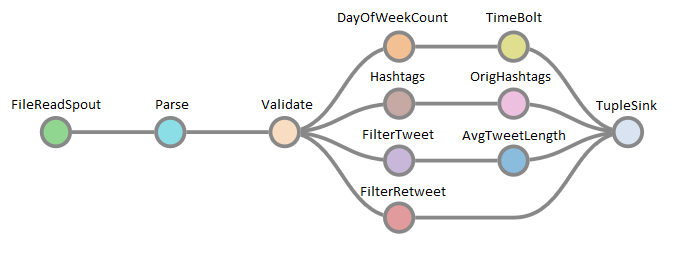
\includegraphics[scale=0.8]{Topologie.png}
\caption{Darstellung der logischen Topologie durch Heron UI.}
\end{figure}

Topologien in Heron besitzen Parameter, durch die der Entwickler deren Verhalten beeinflussen kann.
Für nahezu alle Parameter definiert Heron einen Standardwert.
Im Folgenden werden die Parameter beschrieben, bei der die Evaluations-Topologie vom Standard abweicht.
Die Parameter sind in Tabelle 10.1 mit den zugewiesenen Werten aufgelistet.

Wie schon im vorherigen Kapitel beschrieben wurde die Regulation des Tupel-Stroms deaktiviert.
Die Topologie wurde so konfiguriert, dass jedes Tupel mindestens einmal erfolgreich verarbeitet werden muss.
Deshalb werden Tupel, die in der Folge eines Flaschenhalses verworfen werden, mehrfach von der Quelle ausgegeben.
Dies ist möglich, weil die Bestätigung von Tupel aktiviert wurde.
Dies bedeutet, dass jeder Operator die Bearbeitung des Tupels an die Quelle zurückmeldet.
Erst wenn alle Operatoren die Verarbeitung des Tupel bestätigen, wird das Tupel als bestätigt markiert.
Durch diesen Mechanismus ist es ebenfalls möglich die Latenz des Tupels zu bestimmen.

Die Quelle wurde so konfiguriert, dass ein Tupel, das innerhalb von einer Minute nicht erfolgreich verarbeitet wurde, ungültig ist und wiederholt werden muss.
Außerdem sendet die Quelle maximal 1.000.000 Tupel, ohne dass eines davon bestätigt wurde.
Das bedeutet, dass sich zu jedem Zeitpunkt maximal 1.000.000 Tupel zur Bearbeitung in der Topologie befinden.
Dieser Wert wurde bewusst sehr groß gewählt, um die Ausgabe von Tupeln nicht aufgrund von Flaschenhälsen in der Topologie zu verringern.
So ist sichergestellt, dass die Quelle dauerhaft in der Lage ist Tupel auszugeben, um den realistischen Arbeitsaufwand zu rekonstruieren.

\begin{table}
\caption{Parameter der Topologie}
\begin{tabular}{ll}
\hline
\textbf{Parameter} & \textbf{Wert} \\ \hline
TopologyDropTuplesUponBackpressure & True \\
TopologyReliabilityMode & ATLEAST\_ONCE \\
MessageTimeoutSecs & 60 \\
MaxSpoutPending & 1000000 \\
\hline
\end{tabular}
\end{table}

In der momentanen Version kann Heron die Operatoren nur skalieren, wenn die Tupel zufällig den Tasks der Operatoren zugewiesen werden.
Deswegen wurde diese Konfiguration für die Operatoren der Topologie gewählt.
Außerdem erhält jeder Folgeoperator immer alle ausgegebenen Tupel des Vorgängers.
Es gibt also keine selektive Weiterleitung.
Jedem Task wurde ein CPU-Kern, 1,25 GB RAM und 1,25 GB persistentem Speicher zugewiesen.
Die Topologie wurde mit der Java API von Heron entwickelt.
Diese erlaubt das definieren eigener Logik für die Quelle und die anderen Operatoren.
Im Folgenden werden die einzelnen Operatoren der Topologie beschrieben.

\subsection{Quelle}
Die Quelle ''FileReadSpout'' liest die gesammelten Daten von der Festplatte.
Dies geschieht Zeile für Zeile, was jeweils einem Tupel entspricht.
Jedes erfasste Tupel besitzt einen Zeitstempel mit dem Zeitpunkt, an dem es erzeugt wurde.
Um den Twitter-Datenstrom realistisch nachzubilden wird dabei immer der Zeitstempel des eingelesenen Tupels überprüft.

Um die Topologie auszulasten ist der Datenstrom in der realen Geschwindigkeit, mit der er erfasst wurde, jedoch nicht ausreichend.
Deshalb wird der Zeitraum, in dem die Tupel erfasst wurden, auf einen kleineren Zeitraum komprimiert.
So bleibt die Struktur des Arbeitsaufwandes wie Lastspitzen und Lastabfall erhalten, wird aber in ein kürzeres Intervall geschoben um so insgesamt mehr Last zu erzeugen.
Das Ziel ist, dass in jeder realen Minute in der Evaluation 84 Minuten der aufgezeichneten Daten verarbeitet werden.
Somit werden in einer realen Stunde 84 Stunden der aufgezeichneten Daten abgearbeitet.
Da eine Woche 168 Stunden hat dauert ein Durchlauf der Evaluation 2 Stunden.
Durch die Kompression der Daten, kann ein Arbeitsaufwand erzeugt werden, der die Operatoren so auslastet, dass sie skaliert werden müssen.

Die Quelle wurde so implementiert, dass sie die Tupel anhand des Zeitstempels mit realistischen Schwankungen abgibt.
Dazu speichert sie den Startzeitpunkt der Topologie sowie den Zeitstempel des ersten Tupels in Millisekunden.
Während der Evaluation wird geprüft wie viele Millisekunden seit dem Start der Topologie vergangen sind.
Mit diesen Werten kann der maximale Zeitstempel errechnet werden, mit dem ein Tupel die Quelle verlassen darf.
Der maximale Zeitstempel errechnet sich aus der Differenz von aktuellem Zeitstempel und der Startzeit der Topologie, die mit dem Faktor 84 multipliziert und zu dem Zeitstempel des ersten Tupels addiert wird.
Mit dieser Methode kann nicht garantiert werden, dass Tupel nicht langsamer ausgegeben werden.
Aber es wird verhindert, dass die Tupel schneller als der realistische Arbeitsaufwand ausgeben werden.

Die Leserate vom permanenten Speicher ist in der verwendeten Implementierung wesentlich höher als die Rate des komprimierten Arbeitsaufwandes, sodass eine langsamere Abgabe der Tupel unrealistisch ist.

\subsection{Andere Operatoren}

Um die folgenden Funktionen zu verstehen, sind erst folgende Erläuterungen notwendig.
Ein Retweet ist ein Statusupdate das das Statusupdate eines anderen Nutzers ohne weitere Anmerkung weiterverbreitet \cite{noauthor_docs_nodate}.
Ein Antwort-Tweet ist ein Statusupdate, das auf das Statusupdate eines anderen Nutzers antwortet \cite{noauthor_docs_nodate}.
Ein Tweet zitiert einen anderen Tweet wenn er ihn weiterverbreitet und Anmerkungen hinzufügt \cite{noauthor_docs_nodate}.

Außerdem ist zu bemerken, dass alle Operatoren Tupel direkt weiterverarbeiten und keine Fenster bilden.
Dies liegt daran, dass Heron keine Bearbeitungsdauer der Tupel misst.
Somit können die Modelle der Warteschlangen-Theorie für Operatoren mit Fenstern nicht angewendet werden.

\begin{itemize}
\item{''Parse'': Dieser Operator erhält das von der Quelle ausgegebene Tupel. Dieses enthält einen String, der ein JSON-Objekt beschreibt. Die Daten des JSON-Objektes werden ausgelesen und als getrennte Attribute in einem Tupel weitergeleitet. Löschanfragen für Statusmeldungen werden nicht weitergeleitet.}
\item{''Validate'': Dieser Operator prüft die Lesbarkeit der Daten und gibt sie auf der Standardausgabe aus.}
\item{''DayOfWeekCount'': Hier wird der Zeitstempel des Tupels in den Wochentag, an dem das Tupel erzeugt wurde, umgerechnet. Jedes Tupel erhöht den Zähler für den jeweiligen Tag.}
\item{''TimeBolt'': Dieser Operator gibt den genauen Datumstext für den Zeitstempel des Tupels auf der Standardausgabe aus.}
\item{''Hashtags'': Hier werden die Hashtags des Tweets ausgelesen. In einer Tabelle werden identische Hashtags gezählt.}
\item{''OrigHashtags'': Zählt ebenso Hashtags, allerdings nur für Original-Tweets eines Retweet oder Antwort-Tweet.}
\item{''FilterTweet'': Sendet nur Tweets weiter, die kein Retweet und kein Antwort-Tweet sind sowie keinen anderen Tweet zitieren.}
\item{''AvgTweetLength'': Berechnet die durchschnittliche Länge des verfassten Textes.}
\item{''FilterRetweet'': Sendet ausschließlich Retweets weiter.}
\item{''TupleSink'': Hat keine Operation außer die Tupel final zu bestätigen.}
\end{itemize}

\section{Ablauf}

Für die Evaluation müssen die in dieser Arbeit implementierten Algorithmen die beschriebene Topologie steuern, während sie die Tupel im Zeitfenster von zwei Stunden verarbeitet.
Alle Operatoren starten dabei mit einem Parallelisierungsgrad von eins.
Für jeden der beiden Algorithmen von Lohrmann et al. und Zacheilas et al. wurden fünf Durchläufe gestartet.
Jeder Durchlauf startet, wenn die Topologie aktiviert wird.

Die Hauptsteuerung wurde so implementiert, dass sie alle fünf Minuten die Topologie durch den gewählten Algorithmus prüfen lässt.
Zuerst werden alle Messwerte des Graphen-Modells mit den aktuellen Messwerten aus der Topologie aktualisiert.
Anschließend wurden die folgenden Daten zur Evaluation erfasst:
\begin{itemize}
\item{Minuten seit Beginn der Evaluation}
\item{Sekunden seit Beginn der Evaluation}
\item{Durchschnittliche Latenz der Tupel}
\item{Anzahl fehlgeschlagener Tupel}
\item{Anzahl bestätigter Tupel}
\item{Summe der Parallelisierungsgrade der Operatoren}
\end{itemize}
Der erste Start der Hauptsteuerung erfolgt zur ersten Prüfung, nachdem die Topologie schon 5 Minuten aktiv ist.
Deshalb ist die Anzahl der Minuten und Sekunden seit Beginn der Evaluation um fünf Minuten verschoben.
Wenn alle Messwerte erfasst sind, startet der gewählte Algorithmus und die Topologie wird entsprechend der Empfehlung des Algorithmus skaliert.
Erst nachdem der Vorgang erfolgreich von Heron zurückmeldet wurde, beginnt das Zeitfenster von 5 Minuten bis zur nächsten Prüfung.

Während Heron die Topologie skaliert ist diese gestoppt, sodass während dieser Zeit keine neuen Tupel von der Quelle ausgegeben werden.
Das wirkt sich offensichtlich auf die Zeitbeschränkung für die Tupel-Ausgabe der Quelle aus: 
Die Zeit, die seit Beginn der Evaluation vergangen ist, läuft trotzdem weiter.
Dies spiegelt auch das reale Verhalten wieder, da der reale Datenstrom ebenfalls zwischengespeichert werden müsste, solange die Topologie skaliert.

Während des Vorgangs löscht Heron außerdem alle Messdaten, da die alten Daten für den aktuellen Zustand der Topologie nicht mehr gültig sind.
Nachdem die Topologie wieder gestartet wurde, müssen sich die Zwischenspeicher vor und nach den Operatoren erst wieder mit Tupel füllen, um aussagekräftige Messwerte zu erhalten.
Deswegen ist es sinnvoll erst nachdem die Topologie skaliert wurde weitere fünf Minuten zu warten, damit die Messwerte im System wieder aussagekräftig sind.

Außerdem werden aus diesem Grund bei der Abfrage der Messwerte, die ebenfalls im Intervall von fünf Minuten ausgelesen werden, nur die letzten drei Minuten aus dem CEP-System angefordert.
Dies bedeutet, dass die Messwerte der ersten zwei Minuten, nachdem die Topologie skaliert wurde, weder für die Berechnung des Parallelisierungsgrades noch für die Ergebnisse der Evaluation verwendet wurden.

Die Evaluation stoppt sobald alle Tupel verarbeitet wurden.

\section{Parametrisierung der Algorithmen}

Für die Durchführung der Evaluation mussten die beschriebenen Parameter der Algorithmen definiert werden.
Das Graphen-Modell war so konfiguriert, dass der minimale Parallelisierungsgrad eins und der maximale zehn beträgt.
Die maximale Latenz des Pfades wurde auf 10 ms gesetzt.
Da jeder Task eines Operators eine CPU, und 1,25 RAM verbraucht, konnte aufgrund der verfügbaren Ressourcen der maximale Parallelisierungsgrad nicht höher als zehn gesetzt werden.

Für die Evaluation wurden für den Warteschlangen-Algorithmus die in der Tabelle 10.3 gelisteten Parameter gewählt.
Wie im Original von Lohrmann et al. wurde die Erkennung eines Flaschenhalses ab einer Auslastung von 100\% gesetzt.
Der Koeffizient für adaptives Batching wurde auf null gesetzt, da Heron diese Methode nicht verwendet.
Der Parameter bestimmt ohnehin nur den Anteil der maximalen Latenz des Pfades, der für adaptives Batching reserviert ist.
So kann dieser Anteil auch direkt bei der Angabe der maximalen Latenz berücksichtigt werden, wenn der Parameter auf null steht.
Die Schrittweite des Algorithmus wurde ebenfalls wie im Original auf eins gesetzt.
Die Verwendung des Koeffizienten e wurde deaktiviert, da die gemessene Latenz im Vergleich zu der vom Algorithmus berechneten Latenz sehr hoch war.
Dies hätte wie in Kapitel 7.2.4 beschrieben dazu geführt, dass der Algorithmus sehr hohe Parallelisierungsgrade vorgeschlagen hätte.
Dies hätte in Kombination mit dem maximalen Parallelisierungsgrad von zehn zur Folge gehabt, dass die Topologie während der Evaluation konstant maximal skaliert ist und nie angepasst wird.

\begin{table}
\caption{Parameter für den Warteschlangenalgorithmus}
\centering
\begin{tabular}{ll}
\hline
\textbf{Parameter} & \textbf{Wert} \\ \hline
BOTTLENECK\_THRESHOLD & 1.0 \\
ADAPTIVE\_BATCHING\_COEFFICIENT & 0.0 \\
DELTA\_STEP\_SIZE & 1 \\
USE\_LATENCY\_ADAPTION & False\\
\hline
\end{tabular}
\end{table}

Für den zweiten Algorithmus wurden die in Tabelle 10.4 gezeigte Parametrisierung gewählt.

Die Trainingdaten für den Algorithmus wurden während der Evaluation des Algorithmus von Lohrmann et al. gesammelt.
Alle fünf Minuten, in denen die neuen Metriken aus dem System abgerufen wurden, wurden für jeden Operator die Anzahl eingegangener und ausgegangener Tupel der letzten drei Minuten mit Zeitstempel versehen und gespeichert.
Da die aus der Topologie bezogenen Messdaten vom aktuellen Zustand der Topologie und nicht von den verwendeten Twitter-Daten abhängen, sind auch Fehler reflektiert, die vom Algorithmus von Lohrmann et al. gemacht werden.
Somit ist garantiert, dass die verwendeten Trainingsdaten das Vorhersage-Modell nicht speziell für den vorliegenden Twitter-Datensatz übertrainieren.

Die Hyperparameter wurden für die Evaluation nicht mathematisch optimiert.
Sie wurden lediglich so gewählt, dass die Regression Vorhersagen im richtigen Größenbereich trifft.
Dazu wurden die Zeitstempel sehr schwach gewichtet.
Die Zeit, die seit der Evaluation vergangen ist, wurde stark gewichtet, da sie einen größeren Zusammenhang mit dem Zustand der Topolgie aufweist als der Zeitstempel.
Das Modell für eingehende Tupel beruht nur auf den beiden Dimensionen Zeitstempel und vergangene Zeit.
Daher muss die vergangene Zeit stark gewichtet werden um zu verhindern, dass der Zeitstempel das Modell verfälscht.

Für die Vorhersage der ausgehenden Tupel wurde die Gewichtung des Parallelisierungsgrad so gewählt, dass er sich in etwa gleich wie die vergangene Zeit auf die Korrelation auswirkt.
Wie in Kapitel 8.2.2 erwähnt besitzen der Parallelisierungsgrad und die Zeit, die seit der Evaluation vergangen ist, verschiedene Größenordnungen.
In der Evaluation bewegen sich Parallelisierungsgrade im Einerbereich währen die Zeit bis zu 7200 steigt.
Dies wird durch den gewählten Wert des Hyperparameters ausgeglichen.

Die Kostenfunktion wurde für alle Kostenfaktoren mit eins initialisiert.
Dies fördert die Flexibilität der Topologie, da die Kosten, die Topologie zu ändern, und die Kosten pro verwendeten Task sehr gering sind.
Die Anzahl verpasster Tupel kann jedoch schnell 1000 übersteigen, sodass die Kosten für verpasste Tupel ausschlaggebend für den kürzesten Pfad im Graphen der Zustandsübergänge sind.

Die Vorhersagen wurden für Zeitfenster von fünf Minuten getroffen, um gleich dem Intervall zu sein, in dem die Topologie geprüft wird.
Es wurden jede Runde Vorhersagen für sechs Zeitfenster getroffen, sodass immer Zustandsübergänge für die nächsten 30 Minuten berücksichtigt wurden.

\begin{table}
\caption{Parameter für den Algorithmus mit Regression} 
\centering
\begin{tabular}{ll}
\hline
\textbf{Parameter} & \textbf{Wert} \\ \hline
SIGMA\_INPUT & 1.0 \\
LAMBDA\_INPUT & (1.0, 10000.0) \\
SIGMA\_OUTPUT & 1.0 \\
LAMBDA\_OUTPUT & (1.0, 10000.0 10.0) \\
Kostenfunktion & (1.0, 1.0, 1.0) \\
Abstand Zeitfenster & 300 \\
Anzahl Zeitfenster & 6 \\
\hline
\end{tabular}
\end{table}

\section{Ergebnisse}

Im Folgenden werden für die Beurteilung der beiden Algorithmen die Messwerte verwendet, die während der Evaluation erfasst wurden.
Diese reflektieren kein festes Intervall von fünf Minuten, da die Wartezeit von fünf Minuten jeweils erst nach der Bestätigung, dass erfolgreich skaliert wurde, beginnt.
Außerdem ist zu beachten, dass die gezeigten Auswertungen jeweils zur Minute fünf der Evaluation beginnen, da zu Beginn der Evaluation offensichtlich keine Messwerte vorliegen.
Die folgenden Abkürzungen werden für die Algorithmen verwendet um die Lesbarkeit zu verbessern:
Algorithmus mit Warteschlangen Theorie (WT), Algorithmus mit Regression (RG).

\subsection{Parallelisierungsgrad der Topologie}
Um alle weiteren Messwerte zu verstehen ist es essentiell, dass der Zustand, in dem die Topologie während des Mess-Zeitraums befand, betrachtet wird.
Deshalb wurde jeweils der summierte Parallelisierungsgrad der Topologie gemessen.
Wie in Abbildung 9.3 zu sehen ist, verlaufen die Parallelisierungsgrade unter den beiden Algorithmen sehr unterschiedlich.

Zu Beginn skalieren beide Algorithmen die Topologie nach oben. Es ist ersichtlich, dass WT den Parallelisierungsgrad der Operatoren schrittweise verdoppelt, während RG etwas schneller ansteigt.

Nach dem initialen Anstieg schwankt der Parallelisierungsgrad unter WT sehr stark.
WT nimmt über die Evaluation hinweg viele Anpassungen vor und tendiert dazu, stark zwischen hohen und niederen Werten zu schwanken, da er nur reaktiv auf die letzten drei Minuten reagiert.
Bei hohem Parallelisierungsgrad geht dabei die Latenz der Tupel stark zurück, sodass der Algorithmus ihn verringert.
Ist der Parallelisierungsgrad anschließend niedrig steigt die Tupel-Latenz und der Algorithmus skaliert wieder hoch.
So schwankt die Topologie stark zwischen zwei extremen.
Den Parallelisierungsgrad zu ändern stoppt ebenfalls den Zufluss von Tupeln, sodass diese anschließend in größeren Mengen in die Topologie fließen, was diesen Effekt noch verstärkt.

RG hingegen bewegt sich jedoch sehr konstant und ähnelt der gezeigten Regressionskurve von WT.
Die Ähnlichkeit kann mit der Methode der Vorhersage, die ebenfalls eine Regression ist, zusammenhängen. Obwohl hier ausgehende und eingehende Tupel vorhergesagt werden, hängen diese vom Parallelisierungsgrad ab.
Im Modell von Zacheilas et al. ist nicht explitzit berücksichtigt, dass die Anzahl der eingehenden Tupel ansteigt, sobald Vorgängeroperatoren skaliert werden.
In den Trainigsdaten für die Regression ist dieser Umstand jedoch abgebildet, sodass der Parallelisierungsrad zum Messzeitpunkt der Trainigsdaten Einfluss auf beide Regressions-Modelle auswirkt.

Da die Trainingsdaten immer mit einem bestimmen Parallelisierungsgrad gemessen werden, fällt es RG schwer die Operatoren auf Parallelisierungsgrade außerhalb der erfassten Trainingsdaten zu skalieren.
Für diese Parallelisierungsgrade sind keine Informationen über eingehende und ausgehende Tupel vorhanden und das Regressions-Modell nähert sich eher an bekannte Parallelisierungsgrade an.
Für bessere Vorhersagen ist es daher essentiell, dass Messungen mit allen Möglichen Parallelisierungsgraden der Topologie in die Trainingsdaten mit einfließen.

Wie erwartet, hält der RG Algorithmus den Parallelisierungsgrad konstanter als der reaktive Ansatz von WT.
Einerseits ist die Vorhersagemethode verantwortlich, da dieses einen Mittelwert aus den Trainingsdaten bildet und der Mittelwert konstanter verläuft als die jeweils aktuellen Messdaten, die WT zugrunde liegen.
Außerdem wird bei RG der Zustand der Topologie jeweils für eine halbe Stunde voraus geplant was den Effekt verstärkt.
So zeigt sich fast keine Schwankung, obwohl die verwendete Kostenfunktion eine Änderung der Topologie gleich gewichtet wie das verpassen eines einzelnen Tupels.

Außerdem ist noch zu erwähnen dass der maximale Parallelisierungsgrad von 10 Tasks per Operator nie benötigt wurde.
Somit war dieser Maximalwert kein Flaschenhals für die Topologie.

\begin{figure}
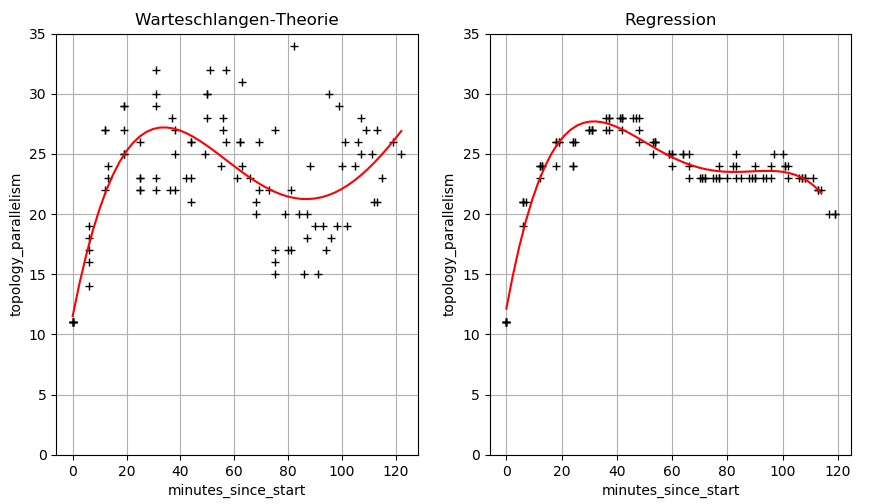
\includegraphics[scale=0.65]{Parallelisierung}
\caption{Parallelisierungsgrade während der Evaluation.}
\end{figure}

\subsection{Latenz der Tupel}

Wenn man den Verlauf der Tupel-Latenz in Abbildung 9.4 betrachtet, kann man feststellen, dass diese sich gegenläufig zum Verlauf des Parallelisierungsgrades verhalten.
Auffällig ist auch, dass die Messwerte von WT im Schnitt deutlich niederer sind, als die Messwerte von RG.

Dies ist durch mehrere Ursachen zu erklären.
Zum einen wird die Topologie wesentlich häufiger durch WT angepasst, als es bei RG der Fall ist.
Wird die Topologie wieder gestartet ist der Fluss der Tupel ungehemmter, als wenn sie konstant läuft.
Dieser Effekt wurde versucht damit abzufangen, dass immer nur die letzten drei Minuten des fünf Minuten Intervalls gemessen wurden.
Trotzdem kann sich der Effekt auf die Latenzen auswirken, da die Topologie eventuell länger als zwei Minuten benötigt bis sie einen stabilen Zustand erreicht.
Des Weiteren ist WT speziell dafür entwickelt die Latenz der Tupel unter einen gewissen Grenzwert zu halten, sodass dies ein essentieller Bestandteil der Steuerung ist.

Jedoch ist festzustellen, dass der gesetzte Maximalwert von zehn Millisekunden für die Latenz des Pfades von WT nicht eingehalten wurde.
Der Grund dafür ist, dass die Berücksichtigung der gemessenen Latenz des Kanals für die Evaluation nicht aktiviert war.
Somit wird die Netzwerklatenz und die reale Warteschlange vor dem Operator nicht berücksichtigt und die berechnete Wartezeit nicht über den Koeffizienten \(e\) angepasst.

Dass der Latenzwert bei RT vergleichsweise hoch ist, könnte daran liegen, dass das Modell eines Operators schlechte Vorhersagen getroffen hat.
Dieser Operator erzeugt dann einen Flaschenhals der die Latenz des Tupels stark erhöht.

Dass die Latenz am Schluss der Evaluation von RT stark ansteigt, könnte daran liegen, dass die Trainingsdaten einen Abfall der eingehenden Tupel gegen Ende aufweisen und deshalb der Parallelisierungsgrad geändert wird.
Diese Struktur der Trainingsdaten wäre damit zu erklären, dass durch die vielen Umstellungen durch WT die Topologie oft gestoppt wird und so über lange Zeit nur die Lesegeschwindigkeit die Ausgabe der Tupel von der Quelle beschränkt.
Dies führt zu hohen Spitzenwerten für die Anzahl ankommender Tupel.
Gegen Ende der Evaluation ist der Verlauf von WT aber weniger schwankend und die Spitzenwerte für ankommende Tupel sinken.
Somit sinkt auch in den Trainingsdaten die Anzahl ankommender Tupel gegen Ende der Evaluation, was den Effekt erklären könnte.

\begin{figure}
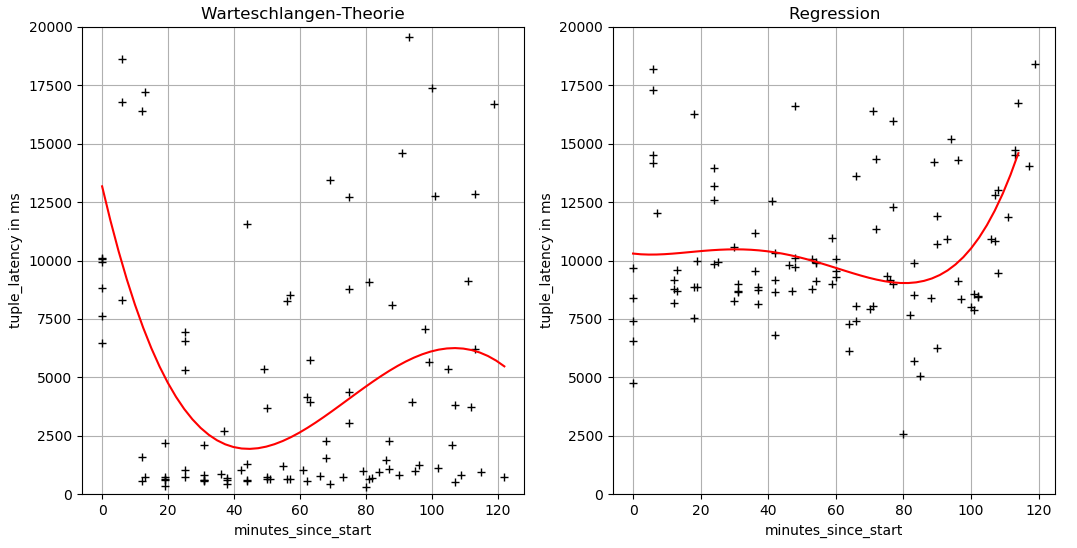
\includegraphics[scale=0.55]{Latenz}
\caption{Latenz der Tupel während der Evaluation.}
\end{figure}

\subsection{Tupel-Fehlerrate}

Zuletzt soll noch die Fehlerrate der Tupel betrachtet werden.
Die Fehlerrate berechnet sich aus dem Verhältnis der Anzahl Tupel, deren Verarbeitung fehlgeschlagen ist, und der Anzahl Tupel, deren Verarbeitung erfolgreich war.
Ein Tupel wird von der Topologie als fehlgeschlagen gewertet, wenn es innerhalb von 60 Sekunden nicht erfolgreich verarbeitet wurde.
In beiden Diagrammen der Abbildung 9.5 ist deutlich zu sehen, dass die Fehlerrate zu Beginn sehr hoch ist.
Erst wenn die Operatoren ausreichend skaliert sind, stabilisiert sich die Fehlerrate.
Für WT ist zu sehen, dass die Fehlerrate sehr oft nahe bei 0\% liegt.
Dies ist dadurch erklärbar, dass fehlerhafte Tupel erneut von der Quelle ausgegeben werden.
Der Algorithmus reagiert anschließend stark auf die erhöhte Anzahl ausgegebener Tupel und kann den Überschuss kurzfristig ausgleichen.
Diese Verhalten wurde in Kapitel 9.7.1 bereits beschrieben.

RG weist hingegen eine sehr hohe Fehlerrate auf.
Dies kann darauf zurückgeführt werden, dass der Algorithmus langfristige Prognosen betrachtet und die erneut gesendeten Tupel nicht kurzfristig ausgleicht.
Zudem basieren die Prognosen auf Messwerten von WT.
WT gleicht die Fehlerrate kurzfristig aus.
Da RG aber auf einem Mittelwert der gemessenen Werte basiert, können diese Spitzen nicht abgefangen werden.

Die hohe Fehlerrate erklärt ebenfalls warum die Latenz der Tupel unter RG in der zweiten Hälfte konstant hoch bleibt.
Im Vergleich zu WT beleibt der Parallelisierungsgrad von RG in der zweiten Stunde konstant und ist somit höher als bei WT.
Allerdings ist die Latenz der Tupel unter RG dennoch höher als bei WT.
Dies erklärt sich durch die konstant hohe Fehlerrate, die nicht abgearbeitet werden kann und somit die Operatoren mit erneut gesendeten Tupeln dauerhaft stark belastet.

\begin{figure}
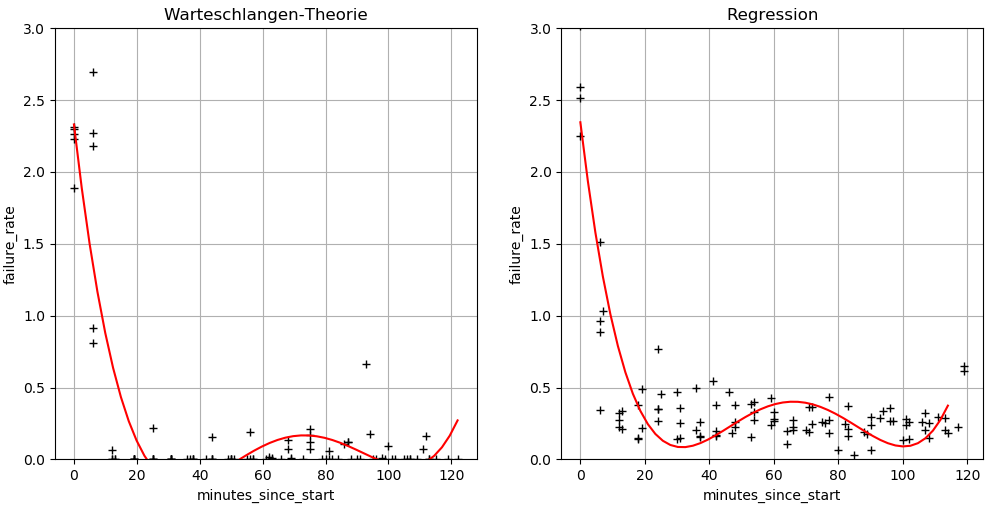
\includegraphics[scale=0.55]{Fehlerrate.PNG}
\caption{Fehlerrate der Tupel während der Evaluation.}
\end{figure}

\subsection{Schlussfolgerungen}

Für das in der Evaluation verwendete Muster des Arbeitsaufwands scheint WT besser geeignet zu sein.
Die Latenz und die Fehlerrate sind beide niedriger als bei RG.
Allerdings benötigt WT zeitweise mehr Ressourcen, die zur Verfügung stehen müssen.
Im Mittel sind die Kosten für Operatoren der Topologie ähnlich.

Da durch die zeitliche Komporession der Daten die Spitzen und Tiefen schneller aufeinander folgen, ist es erklärbar, dass WT durch die eher kurzfristige reaktive Herangehensweise besser auf die schnelle Abfolge der Extreme reagieren kann.
Dies setzt allerdings voraus, dass die ankommenden Tupel während der häufigen Änderungen der Topologie zwischengespeichert werden können.
Der Algorithmus von Lohrmann et al. konnte, trotz vielen Änderungen an der Topologie, den Rückstand, der Tupeln die bearbeitet werden müssen, ausgleichen.

Der Algorithmus von Zacheilas et al. ist relativ stark an die Mittelwerte der Trainingsdaten gebunden.
Damit der Algorithmus erfolgreich eingesetzt werden kann, ist es notwendig, dass Messdaten für möglichst viele Parallelisierungsgrade eines Operators vorhanden sind.
Sind die Daten nicht vorhanden, dann unterscheiden sich die Vorhersagen für hohe und niedere Parallelisierungsgrade nicht stark genug.
Durch eine Optimierung der Hyperparameter kann diesem Verhalten ebenfalls entgegengewirkt werden.

Ein weiterer Punkt ist, dass RG den letzten Operator der Topologie nie skalieren wird, da die Anzahl der ausgegebenen Tupel immer null entspricht.
Somit ist die Anzahl verpasster Tupel des Operators und die damit verbundenen Kosten immer null.

Für einen Workload der wenige Ausreisser besitzt und sich eher moderat verändert wäre der Algorithmus von Zacheilas et al. vermutlich besser geeignet als der Algorithmus mit Warteschlangen-Theorie. 

